\chapter{Functionality of RFID technology, NoSQL technology}
\label{Kap2}

The second chapter is divided into two parts: the functionality of RFID technology and NoSQL technology. In the first part, several characteristics of the used RFID technology and the components of a RFID system (see section \ref{rfid_technology}) are depicted. Concerning the security and privacy of RFID systems, section \ref{secprivrfid} refers to some useful methods against threats. After that, in the second bigger part \ref{nosql}, some general information about NoSQL is given and compared to SQL technologies. Finally, the term 'Big Data' is introduced and discussed briefly in section \ref{bigdata}. 

\section{RFID technology} \label{rfid_technology}

According to Ajami and Rajabzadeh \cite{ncbi}, RFID technology is capable of an automatic unambiguous identifiation without being placed in the \ac{LOS} of their objects. The data between RFID tags and readers is transmitted through radio waves. An early RFID-like technology was used as early as in 1940's to identify airplanes during Second World War. Today, it is used in several different areas, like for example in manufacturing, supply chains, agriculture, transportation systems, healthcare services etc. 

\subsection{Components of an RFID application} 

Ajami and Rajabzadeh \cite{ncbi} mention five main components existing in a RFID system. First, there is the RFID tag attached to an object ensuring its unique identification. Second, the RFID reader detects each tag and generates a response: an electromagnetic wave is sent back to the RFID reader from the detected RFID tag, conveying the RFID information onto that wave. In order to detect tags, one or more antennas (third component) have to be connected to a reader. Fourth, in every RFID system has to exist a communication infrastructure which enables the interaction of readers and tags through an \ac{IT} infrastructure. Last, to enable users to connect to the RFID infrastructure and to control its modules, there has to be established an application software including an user interface and a backend service (e.g. database).

\subsubsection{RFID tags} \label{tag}

With regard to the variety of RFID tags, three fundamental types are distinguished: Active, semi-active and passive RFID tags \cite{henrici} which all consist of an antenna, a microchip and packaging. Active RFID tags consist of a microchip and have their own power source. As a characteristic, they are more expensive than the other two types. After that, semi-active tags or also called 'hybride' tags have their own power supply which is only used to support the microchip. The transmission or communication between semi-active tag and reader is implemented by using the power of the reader's field. Finally, the passive RFID tags do not consist of a power source and only work in the reading range of the reader. They harvest their needed energy from the electromagnetic field of the reader and are cheaper than active tags. Moreover, passive tags are lighter than active tags and provide a long-lasting service. In constrast to active tags, passive tags are limited in their read range and functionality.

The 'EPCglobal', an industrial consortium, proposes another kind of RFID transponders (tags) classification, distinguising between five classes of RFID transponders (tags) \label{classes} \cite[p.15 ff.]{fokus}. The first three classes include passive tags which have no own energy or power supply whereas the last two classes are used to identify active tags. Particularly, the 'Class 0' signifies that the serial number is written during production process. The 'Class 1' means that a transponder can only be labelled once. 'Class 2' means the tag is rewritable, e.g. the serial number or further data can be rewritten. 

'Class 3' represents the tags which have their own internal battery for a microchip but whose data exchange (sending and receiving information and messages) is supported by the reader's energy. With respect to the last two classes, Tamm and Tribowski remark the purpose of reassessment, aggregation and transformation of RFID data. Actually, these active tags are no 'real' RFID transponders but 'telemetry transmitter' because they do not influence the electromagnetic field of the reader and do have their own electromagnetic field. In particular, 'Class 4' refers to tags which have their own power supply which is used for the microship and data exchange. Furthermore, they cannot communicate with passive transponders. The final 'Class 5' appoints to tags which can also communicate with passive transponders. 

According to Henrici \cite{henrici}, the memory capacity of passive RFID tags can vary from single bits to kilobytes which is not much. As a recommendation, an external database to store tag-specific data should be used. For instance, a memory of 12 bytes is very common to store \ac{EPC}. Concerning the memory technology, Henrici distinguishes two general types of storage: non-volatile and volatile storage. Non-volatile storage can be divided into read-only (fixed after manufacturing), \ac{WORM} and read-write which set the access privileges to the memory. The opposite of non-volatile storage is called volatile storage and is used for example to perform calculations after power-up. Besides, Henrici mentions tags which are able to check passwords or implement ciphering algorithms to ensure data privacy.

To maintain the security and authenticity of each RFID tag, Henrici \cite[p.93 ff.]{henrici} depicts four implementation methods of identification. 
The first and easiest method is called 'regular identification'. It implies that each tag sends its complete identifier to the reader within a \ac{SMLE}. Another method is called 'implicit identification'. It uses information that has not been provided explicitly for particular identification purpose. Thirdly, a more sophisticated and secure method to identify tags which is the 'multistep identification' method. As the name of this method is very self-explaining, one should image the next three identification steps: In the first step, only parts of the identification information is revealed. After that, an authentication and authorization step follows. Once, being authenticated and authorized, more identification information will be revealed. 

Other than the mentioned methods, Henrici describes a very secure method to identify tags which he calls 'encryption and shared key identification'. As an advantage, this identification method protects every information contained in an identifier which can be transmitted in encrypted form. The vast amount of information requires a high internal storage of the tag, like given by active tags. To arrange an encrypted transmission of the information from passive, low cost tags the identifier needs to be calculated outside the tag and then stored on the tag (directly in enciphered form). So, there would be no additional expenditure to enable encrypted and shared key identification. 

\begin{figure}
\centering
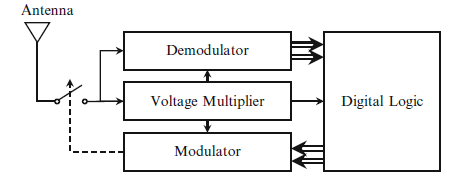
\includegraphics[width=\textwidth]{rfidtagdesign} 
\caption{\label{fig:tagdesign}Elements of a RFID tag \cite[p.13]{chipless}} 
\end{figure}

As above mentioned, RFID tags can be categorized in different ways. In contrast to Tamm and Tribowski \ref{classes}, Rezaiesarlak et al. \cite{chipless} describe three different categories \cite[p.9 ff.]{chipless}: First, RFID tags can be distinguished between inductive and radiative (or backscattering-based) tags. Inductive tags are the ones which work below a frequency of 100 MHz and their operating principle is based on inductive coupling between the reader and the tag coil-like antennas. Radiative tags work in the UHF (300 - 3000 MHz) frequency band, providing more reading range as no coupling between reader and dipole-like tag antenna is required. Second, there can be differentiated between active and passive tags as mentioned above. Last, there are both chipped and chipless tags. 

\subsubsection{RFID readers} \label{reader}

In this section, RFID readers will be explained in detail. 
To start with, one has to imagine existing objects which are tagged with a RFID tag. To implement functionality to these tags and to connect them to a middleware or a backend system, a detector is needed. This detector is the RFID reader which consists of an antenna, a power supply (for passive tags), a microprocessor (to control devices) and an interface for forwarding data to the processing backend system \cite{henrici}. 

Generally, two different types of readers can be distinguished: Stationary and mobile readers. Stationary readers need to be integrated into the existing system architecture by additional middleware \cite[p.133 ff.]{mobile}. Likewise, direct coupling between application systems is not possible because of the amount of data which has to be handled, the lacking ability of being a real-time system and the limited possibilities of RFID readers to produce the required process information. To give an example of the use of stationary readers, they are oftenly used for goods receiving or stock management. Furthermore, stationary readers are fixed to a specific location and need permanent network connection. Additionally, the antenna and reader are spatially separated from each other \cite[p.17 ff.]{fokus}.

On the opposite, mobile readers do not need permanent network connection. They can be used for example to query prices in a supermarket (of those products tagged with RFID tags). Usually mobile readers are integrated into mobile devices, connected to laptops, \ac{PC} or tablets. To connect themselves to an existing system, mobile RFID readers need a device driver which enables the communication between reader and the installed application on the device \cite[p.133 ff.]{mobile}. Furthermore, the antenna as well as the reader itself are integrated into their casing \cite[p.17 ff.]{fokus}.

Nevertheless, there is the possibility of conntecting several antennas to one reader to extend the range of field.
As mentioned in the section before \ref{tag}, RFID tags and readers communicate via electromagnetism. The reader's detection range depends on the frequency as well as the electromagnetic field \cite{henrici}. In general, four frequency ranges can be differenced: \ac{LF} (125-134 kHz), \ac{HF} (13.56 MHz), UHF (868 MHz-915 MHz) and Microwave (2.54 GHz-5.8 GHz). Each frequency range has its own physical characteristics, such as the mechanism to send/receive information from/to antennas and tags (backscattering, electromagnetic coupling) or the reading range.

According to Vizinex \cite{vizinex}, an american company located in Pennsylvania (U.S), HF tags can be used for short read ranges (up to 8 cm). They are usually tagged to tissue samples, blood and critical fluids. Furthermore, HF tags work well in proximidity to liquids as well as human tissues. UHF tags provide longer read ranges and can be detuned by proximity to tissue, fluids and metals. These tags are typically used to track and locate critical medical devices, manage inventories of medical items and track as well as identify patients. Moreover, UHF tags are compatible with worldwide standards and easily deployed because of the compatibility with widely available and competitively priced RFID readers.

The functionality of passive tags within near field is different from passive tags in far field. In near field, the operating principle to send/receive information is based on electromagnetic coupling between the tag and the reader. That means that only one RFID tag can be read simultaneously. It also defines the kind of antennas to be used (typically coils). 

This mechanism does not work in far field where the interrogation signal is backscattered by the RFID tag  \cite{henrici}.
All in all, readers are able to query tags and to read and write tag data. But the storage of information and the information processing does not take place in readers or tags, but in the middleware or backend systems. These will be explained in the next paragraph.

\begin{figure}
\centering
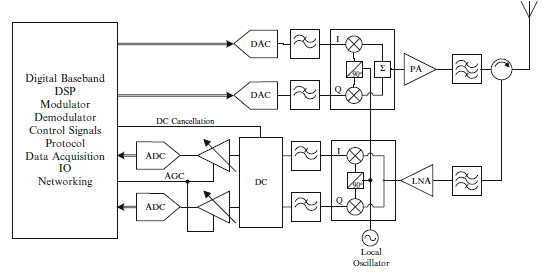
\includegraphics[width=\textwidth]{rfidreaderdesign} 
\caption{\label{fig:readerdesign}The design of a RFID reader \cite[p.17]{chipless}} 
\end{figure}

\subsubsection{RFID backend systems} \label{backend}

As Henrici \cite{henrici} mentions, the backend can be divided into two parts: Middleware and applications. Both of them run on the same computer within the same network which is important for the permanent connection to RFID readers and all existing tags. The advantages of a middleware in this use are that no adaption of appications is needed, an open and neutral interface for other applications is provided. Besides, as the middleware is used to aggregate and filter data, the tags only have to identify objects. As a result, modularity of the system is maintained.

The RFID middleware can be defined as follows: '[...] the software component for preparation and deployment of RFID data which enables the integration of RFID readers and further infrastructure into the operational application systems [...]' \cite[p.20 ff.]{fokus}. According to this definition, there have to be considered three fundamental functions of the middleware: Reassessment, Aggregation and Tranformation. 

To start with, during the reassessment, all received data from the antennas can be redundant or flawed. This redundancy is caused by different antennas detecting the same RFID transponder at a time or because one RFID transponder has been detected multiple times during one time frame. Flawed means that transponders were not detected in the intended field or they were detected incorrectly. In second place, aggregation defines the process of summaring all contextual information into one single RFID information ('together into one'). In third place, the term 'transformation' is used by syntactic and semantic means. 

To come to a conclusion, the RFID middleware improves the management of readers by abstracting from technical details. Furthermore, it provides a scalable solution which reduces the unneeded complexity which is transmitted to the users \cite[p.20 ff.]{fokus}.   

Concerning the data management of RFID systems, Tamm and Tribowski suggest three general concepts of storing tag-specific data: 'Data-on-Tag', hybride forms and 'Data-on-Network' \cite[p.22 ff.]{fokus}. 'Data-on-Tag' is a highly recommended method because of the decentral data storage. It improves the user's privacy accessing object-referred information. Moreover, the 'Data-on-Tag' strategy is useful if only relevant and necessary information are contemporarily needed. In addition to that, if the system is not available, the processes can be executed with the tag's information.
Furthermore, 'Data-on-Tag' brings many advantages with it like for instance a raised reliability of the entire system because the processes are decoupled from central system components. 

On the contrary, 'Data-on-Network' implies a central data storage. Further, it can be easily standardized because only the identification number has to be standardized. Further, the only additional requirement remains the working network connection. Mentioning the different data storage concepts in RFID systems brings up another term which is used to detect e.g. product piracy: \ac{CEP}. CEP uses compound read events to detect the multiple capture of one identification number (at different places). If multiple captures of the same identification number are found, the mechanism concludes to a copy of the RFID transponder. 

Actually, data is barely stored on RFID tags because of the limited resources in low-cost tags. It is recommended \cite{henrici} to store tag information on an external database. As an advantage, databases provide high flexibility to change data or to execute queries without the tags being present. Furthermore, the backend infrastructure should use a \ac{SSL} or \ac{TLS} protocol to ensure a secure transmission of data. Finally, the data would be transmitted and stored in a backend infrastructure on a central storage \cite{henrici}.

\subsection{Functionality of RFID system}

When developing an RFID system, it is important to think about the unique identification of each object. To enable a reliable identification of objects, only one RFID tag should be attached to each object. The tag itself has a 'read-only' or in some cases 'rewrite' internal memory which enables users to get or change the object's information \cite{ncbi}. 

Secondly, the RFID reader generates magnetic fields to enable the RFID system to locate objects (via tags) within its range. Additionally, the high-frequency electromagnetic energy and the query signal which is generated by the reader triggers tags to reply to the query. Each query can have a frequency of 50 times per second \cite{ncbi}. Thus, it is possible to generate large quantities of data which have to be filtered by supply chain industries. 

Each filter is routed to a backend information system, using a software similar to 'Savant' which is used to control the data. 'Savant' acts like a buffer between the HIS and the RFID reader \cite{ncbi}.
Besides, Tamm and Tribowski \cite[p.18 ff.]{fokus} distinguish between three classifications of RFID systems: 'Close-coupling-systems' ($\le1m$ range), 'Remote-coupling-systems' ($\le1m$ range) and 'Long-range-systems' ($>1m$ range). 

\subsection{Security and Privacy of RFID systems} \label{secprivrfid}

Security and privacy in the healthcare sector is a very important and highly discussed issue. As these are very large issues, which could not be described within a few paragraphs, there will be depicted some examples of threats. In the second section 'Solutions and Methods against Threats' \ref{solution}, five important recommended countermeasures will be described. 
At this point, especially the term of privacy should be defined clearly. According to Tamm and Tribowski \cite[p.90 ff.]{fokus} privacy stands for the right of an individual to keep certain aspects of his life private. Aspects refers to the informational self-determination which should not be controled by further instances, like e.g. systems or third-parties. Additionally, privacy is considered as basic right which is also defined in the Federal Data Protection Act and includes explicitely the protection of personal data.

\subsubsection{Security Problems and Threats} \label{problems}
 
As Henrici \cite{henrici} mentions, there are two fundamental fears about the RFID technology. The first fear concerns marketing purposes, such as creating very detailed customer profiles which lead to a vast amount of information. Secondly, the technology offers the possibility to keep people under surveillance which implies advantages and disadvantages. As an advantage, the patients' life gets more confortable and companies will be more productive. As a negative result, people's privacy is violated and the application's security is not addressed properly.

Aside from the two fears, Henrici describes several risks of RFID systems, such as the ease of disrupting the service which indicates data security and privacy problems. When talking about security, one should distinguish between security of systems and services and the security of data and information. The last point can only be ensured by secure systems \cite{henrici}. 

In the following, some security and privacy risks using RFID technologies will be explained. To start with, one should think of his passport and the data which is stored on it. The new passports have an internal RFID tag which enables readers nearby the passport to read out all data and to copy them as well. Since passive RFID tags do not have their own power supply, they can be read through a nearby reader. So, reading out the passport's data would not be very complex.
Moreover, Henrici mentions product counterfeiting in pharmaceuticals which can cause a lot of harm, like the death of patient's. Nevertheless, the drug market is bound to strong regulations, like for example through the \ac{FDA}. To detect and reduce product counterfeiting, RFID tags need to prove genuineness of original products to patients and should inhibit cloning them.

In his book, Henrici mentions six cases of possible attacks to RFID systems \cite[p.31 ff.]{henrici}. The first attack is called 'Illegitimate reading of data' and describes the possibility of side-channel attacks which use the communication protocol between passive tags and backend systems. As described in section 'RFID backend systems' \ref{backend}, passive tags are used more often and are less expensive than active tags. Nevertheless, the vulnerability of synchronizing each tag with the backend system through a protocol enables attackers to bypass normal protocols so that they can readout all transmitted data.

The second possible attack, Henrici mentions, is called 'eavesdropping of data'. It is caused by the problem of the public and shared communication channel between readers and tags. Compared to 'illegitimate reading of data', everybody near enough the communication channel is able to eavesdrop the conversation because of the use of passive tags. Particularly the 'forward' channel from reader to tag has a stronger magnetic field than the opposite direction which makes it more easily being eavesdropped than the backed one. 

Thirdly, Henrici declares 'cloning or mimicking of tags' as a third threat. His definition of cloning a tag is restricted to creating an exact logical copy of an item which is not distinguishable from the original tag on the protocol level. There might exist some minor differences like the power consumption or time response but the replica cannot be detected with ordinary readers but only with appropriate equipment. The second term 'mimicking' defines the action of infiltrating incorrect data into the RFID system. To show an example, the location might be used for authentication of items. By mimicking a tag, the location can be manipulated and items might appear where they do not exist in reality.

Fourthly, 'recognition of objects' represents another possible threat of RFID systems. In particular, when persons have been detected, they can be used to explore customer habits. Or, in case of patients who wear implants, these might be recognized and the medical information stored on each implant might be abused. In general, each person who carries objects with affixed RFID tags, like wristwatches, shoes etc. might be recognized by an attacker.

Next, the possibility 'tracking of objects' should be considered carefully since tracking of persons can cause many privacy violations. Henrici distinguishes two types of tracking: The first one is called 'direct mapping' and refers to the tracking of RFID wristwatches or glasses. 'Direct mapping' is only possible when the distance between detector and tag is short and the do not exist many tags in one place. Failing that, other items might be tracked by detecting their constellations to each other. These constellations can lead to unwanted creation of movement profiles and the abuse of infrastructure for surveillance by a totalitarian government.

Lastly, Henrici defines the threat of 'causing malfunction' which means that attackers (after having abused one of the above mentioned possibilities) are able to render RFID system malfunctioning. This malfuncionting can be revealed by physical destruction or chemical treatment of tags.  

\subsubsection{Solutions and Methods against Threats} \label{solution}

First of all, data security should always be maintained by the RFID system. But what are the exact countermeasures to prevent an attack on an existing RFID system? When Henrici \cite[p.64 ff.]{henrici} talks about solutions and methods against security threats, he calls them 'Goals of Security and Privacy'. In his book, these goals refer to the possible attacks or threats mentioned in section 'Security Problems and Threats' \ref{problems}. In the following, the countermeasures will be explained. 

'Illegitimate reading of data' can be prevented by controlling data access and ensuring data integrity in RFID systems. False data should be infiltrated because of illegitimate access.
'Eavesdropping of data' can be coped with implementing means for detection and recovering so that the system should keep running even if attackers try to put it out of service. Besides, the integrity of system should always be kept. Another strategy preventing eavesdropping is to maintain data security. Henrici defines a 'good' RFID system to be able to cope with illegitimate reading of data and to treat all the data confidentially.

'Cloning or mimicking of tags' which can be compared to counterfeiting can be prevented by using authenticity mechanisms to identify specific tags. Therefore, RFID tags that can prove their own authenticity should be preferred.

Unwanted 'recognition of objects' can be avoided by developing technical models that provide suitable trade-off of functions. If a function is not wanted by the user, e.g. to allow everyone in the surroundings to read out all RFID attached object, he can adjust this by defining different user roles and rights.

Regarding the realization of the above mentioned goals, there are many challenges which have to be faced. Henrici \cite[p.66 ff.]{henrici} describes four general challenges which will be explained in the next paragraph. 

First of all, since there are different parties, like e.g. logistic companies and customers which have different needs, the developer has to meet all of their requirements. For instance, the different user needs might be realized by developing different views which depend on the particular user role.

Second, developing a secure RFID system is a multidisciplinary challenge \cite{henrici} including six different departments: Computer science (designing communication protocols and the middleware), electrical engineering (realizing the required functionality in hardware and physical layer of communication between tags and readers), mathematics (developing basic cryptographic primitives and theory of probabilities for different areas), economics (adapting the application's constraints imposed by laws of market and assessing real world applicability of approaches), social sciences (including user's requirements, such as privacy and usability) and law (maintaining a legislative basis among people and organizations).

Third, there are more requirements to be faced than 'only' security and privacy, such as low costs or coping with few capabilities and resources. Besides, the enrollment of an RFID system, e.g. in a hospital with many distinctive departments, leads to an inter-organizational operation. To implement this inter-organizational operation, several standards have to be integrated. 

Finally, additional requirements have to be considered: Scalability of the system, dependability, low complexity of system, robustness, transparency and usability etc. Henrici claims, that the safeguards should not limit the read range and the speed of reading. Moreover, when using cryptographic primitives, migration paths should be considered.  

\section{NoSQL technology} \label{nosql}

\subsection{Characteristics of NoSQL Databases}

There are many possibilities to store data from application systems. \ac{SQL} can be seen as one of the fundamental database technologies used since the 1980/1990ies \cite[p.137 ff.]{nosql_meier}. The technology of SQL offers advantages, such as consistency, security and integrity of data, as well as the protection of transactions. On the other side, there come along many disadvantages while using SQL. 

To give an example, checking the integrity of data in case of a higher amount of data implicates the need of a higher processing power. Furthermore, facing large-scale development, the efficiency and performance of SQL based systems are decreasing. Moreover, the flexibility and data handling demonstrates another challenge when using SQL. Actually, in practice, the performance is often more important than the consistency, e.g. in social media.    

In the past ten years, there were some NoSQL database technologies coming up. In 2000, these databases were called 'Web-Scale-Databases' because of the need of data storage systems which should handle with the large amount of data of web services \cite[p.221 ff.]{nosql_meier}.

The term NoSQL can be understood as 'Not only SQL' which signifies extension of the existing SQL functionalities. Some data specialists prefer the context of 'no relational databases' which is controversial because of the use of graph databases which deal with relations between nodes.   

In the next section, some examples for the NoSQL data management will be explained and compared to the usual SQL data management. According to Meier and Kaufmann \cite[p.3 ff.]{nosql_meier}, SQL databases are formed on a relation-based model which contains tables with entries. Furthermore, each entry has attributes which are defined by a validating range. A table is defined by its table name, the attribute's name and an identification key. It can have both a column or row order or none of these. The relational model indicates that every table is a set of random tuples and that the relations between data is realized by using tables. The result of SQL queries are always tables which can be uniquely, minimally identified by their identification or primary key.

In contrast to that, the technology of NoSQL offers more possibilities to store data, like for example in key-value stores, column stores, document stores or graph databases \cite[p.16 ff.]{nosql_meier}. These four types of NoSQL databases are also called 'Core-NoSQL-Models'. Besides, other NoSQL database models like object databases, \ac{XML} databases or grid databases are defined as 'Soft NoSQL Models'. 

To give some examples of the 'Core-NoSQL-Models', their fundamental characteristics will be described in the following. The key-value stores (e.g. Cassandra) provide the simplest way to store data by using an identification key and a list of values. Document stores (like e.g. MongoDB \ref{mongodb}) store the data in form of structured text data like \ac{JSON} or XML. In contrast to key-value stores, document stores have a pre-defined structure but are schema-free which means that the data structure can be changed over the time. 

Graph databases (e.g. Neo4J) introduce a new way to store data: It introduces a graph-based model. Each graph consists of nodes and edges which connect the edges and demonstrate their relations. Each node can have concepts and object. Both, nodes and edges have a label and can contain properties. Each property contains an attribute and a value. The query language for graph databases is called 'Cypher' \cite[p.16 ff.]{nosql_meier} which is a declarative language. Users of Neo4J and other graph databases are able to specify their retrieval query by defining nodes and edges. By evaluating all possible paths (or connections between nodes and edges), the database system calculates all requested patterns.   

Generally, NoSQL technologies are popular for their high availability as well as their protection against system failures by using different replication concepts, e.g. 'Consistent Hashing' \cite[p.11 ff.]{nosql_meier}. In addition, NoSQL is characterized by its vertical and horizontal aligned scalability, its weak or non-existent restrictions concerning schemas and data models. Along, NoSQL databases offers simple data replication and easy access through API \cite[p.221 ff.]{nosql_meier}.  

Edward and Sabharwal discuss the pro and cons of NoSQL technologies in their book \cite[p.17 ff.]{mongodb_edward} which will be given in the next paragraph.
On the one hand, NoSQL offers high scalability, manageability and administration (such as automated repairs, distributed data etc.), low cost and flexible data models. But on the other hand, using NoSQL factors like maturity, limited query capabilities, administration (installing and maintaining solutions) and limited expertise (developer and administrator community are limited).

A \ac{DBMS} defines a software which describes, stores, queries data independently from an application \cite[p.2 ff.]{nosql_meier}. It consists both of a storing and managing component. The storing component is composed of all data which has to be stored in organizational form and their description. The managing component contains a querying or manipulating language to evaluate data and to change them, such as access control units and an user interface. Concerning the use of web applications and a heterogeneous data pool in real-time, SQL databases are often not suitable for these problems. In this case, a NoSQL database should be considered. 

\subsection{Excursus: Big Data} \label{bigdata}

The term 'Big Data' has been emerged during the past 10 years. Due to the enormous data pool, e.g. in social networks or user analysis, which is not easy to manage with usual software tools, new data technologies were needed. As a solution, NoSQL technologies have been arised. Furthermore, Big Data refers to unstructured data which comes from different sources \cite{nosql_meier}. 

Edward and Sabharwal define Big Data as the following: It is a '[...] term used to describe data that has massive volume, comes in a variety of structures and is generated at high velocity. This kind of data poses challenges to the tradtitional \ac{RDBMS} used for storing and processing data. Big Data is paving way for newer approaches of processing and storing data.[...]' \cite[p.1 ff.]{mongodb_edward}. Furthermore, Edward and Sabharwal refer to an explosion of data created by smartphones, social networking sites, in short words from various sources in various formats, such as video, text, speech, log files and images. The type of stored data varies by its 'sector', e.g. retail and whole sale, administrative parts of government, financial services mainly generate text or numerical data (including customer data and transaction information). 

On the other hand, in the healthcare, manufacturing, media and communication sector especially multimedia as well as image data is produced. To give an example, X-Rays, CT and other scans dominate the storage volumes in healthcare. 

Another important point concerning large amount of data is the 'consumation model' or data handling, that is, how data is managed depending on the different parts involved \cite[p.6 ff.]{mongodb_edward}. Edward and Sabharwal declare two models: In the old model, few companies produced data and all others (users, clients, etc.) used them, similarly to a broadcasting-like model/system. But nowadays, they claim that '[...] all of us produce data and all of us consume them [...]' \cite[p.6 ff.]{mongodb_edward}. This creates a new challenge of developing multiple user data models and make the existing data management system more scalable than in the past. 

\subsubsection{Velocity, Variety, Volume}

When talking about Big Data, three concepts have to be highlighted: Velocity, Variety and Volume.

Velocity refers to the real-time high-speed evaluation of the upcoming data \cite{nosql_meier},  also known as 'real-time insight' \cite{mongodb_edward}. Edward and Sabharwal describe velocity as 'Data in motion' \cite[p.7 ff.]{mongodb_edward}. Besides, they mention that if data cannot be processed at required speed, it losses its significance. For many companies and organizations, it is very important to process data both when it is moving as well as when it is static. 

Variety means that there are distinct formats of data: structured (e.g. integer, string), semi-structured and unstructured data \cite{nosql_meier}. Edward and Sabharwal describe variety as 'Data in many forms' \cite[p.7 ff.]{mongodb_edward}. As mentioned in the last paragraph, data can vary from simple text files, log files, streaming videos, photos, meter readings, stock ticker data, PDFs and many other unstructured format.   

The last characteristic of Big Data, volume, deals with the high amount of data \cite{nosql_meier}. Edward and Sabharwal describe volume as 'Data in many forms' \cite[p.7 ff.]{mongodb_edward}. They see a reason for the higher volume in businesses becoming more transaction-oriented and the number of transactions is increasing. Moreover, more devices are connected to the internet which increases the size of data.

Calolas et al. refer to challenges like e.g. dealing with tremendious amounts of data, unstructured data (diversity of \ac{OSN}) as well as the complexity to challenge analyzing social networks data \cites{trends_nosql}.

\subsubsection{Usage of Big Data}

Edward and Sabharwal depict five large use cases of Big Data which will be explained now \cite[p.9 ff.]{mongodb_edward}. Firstly, visibility of data is very important for many companies. For example if data is accessible across departments of a company, it can be readily integrated. This reduces the search and processing time, improves product quality according to present needs \cite[p.9 ff.]{mongodb_edward}. 

Second, discover and analysis information is another use case for large amounts of data. After capturing detailed data, e.g. of inventories, employees or customers, new information or patterns will be discovered and analyzed. The captured information and knowledge can be used to improve processes and performance of companies \cite[p.9 ff.]{mongodb_edward}. 

Third, segmentation and customizations can be effected by means of using Big Data. To give an example, the segmentation of customers is based on various parameters and can aid in targeted marketing campaigns or tailoring of products to suit the needs of customers \cite[p.9 ff.]{mongodb_edward}. 

Fourth, Big Data can aid, improve or automize decision making by using Big Data analytics which can minimize risks and uncover valuable insights. Lastly, Big Data can strengthen innovations in existing products by using data gathered for actual products \cite[p.9 ff.]{mongodb_edward}.    

\subsubsection{Big Data challenges}

The issue 'Big Data' not only offers many possibilities or use cases, but also faces many challenges \cite[p.11 ff.]{mongodb_edward} which will be discussed in the consecutive paragraph. To start with, Edward and Sabharwal indicate policies and procedures which can constrain the use of Big Data. They refer to data privacy, security, intellectual property of organizations. Furthermore, in order to comply with various statutory and legal requirements, Big Data has to face the challenge of data handling, which includes issues around ownership and liabilities around data. In second place, the access to data has to be controlled precisely.

Since some data might be available to third parties, the gaining access poses a legal, contractual challenge. After that, in order to handle Big Data, new tools as well as technologies have to be built specifically. Moreover, there might exist legacy systems in several organizations or companies which have to deal with Big Data. Besides, there is a lack of experienced resources in these newer technologies which is also a challenge to.

Most of the legacy systems are designed to work with structured data \cite[p.11 ff.]{mongodb_edward}. Since legacy systems are created to perform fast queries and analysis on tables and columns, they cannot be used to hold or process Big Data (which contains unstructured data). Another important point is the data storage for Big Data. Currently, in many companies, data is stored on big servers (using \ac{NAS} or \ac{SAN} systems) \cite[p.11 ff.]{mongodb_edward}. With the increasing data, the server size and backend storage size has to be increased. 

Lastly, when handling with Big Data, data processing is very important . Usual algorithms in legacy systems are designed to work with structured data and are limited by data size. Therefore, legacy systems are not capable of handling processing of unstructured data, high volumes of data, speed etc. To capture value from Big Data, the deployment of newer technologies are needed. 

\subsubsection{Big Data technologies}

Edward and Sabharwal propose several ways of implementing Big Data technologies \cite[p.12 ff.]{mongodb_edward} which will be depicted in this paragraph. To begin with, Big Data needs new storage and processing technologies which are designed for large, unstructured data. After that, other technologies like parallel processing, clustering are emerging in order to handle Big Data. Additionally, large grid environments, high connectivity and high throughput offer new fields for software developer and data scientists. Finally, cloud computing and scale-out architectures have been arised during the last years.